\chapter{Logic Implementation with JavaScript} \label{chapter:desgin}

The logic of this app is divided into two parts. First part is JavaScript logic, that is responsible for the functionalities of each HTML site, more precisely, the dynamic response to the user. Second part is Java Android logic, which is responsible for the main function called car tracking and all other functionalities that could not be accomplished with help of JS. 
\\

Altogether there are 10 HTML sites and each one of them has some functionalities that had to be implemented with JS or Android Java. A simple example of a functionality is pressing a button. This button triggers a function inside the JS. 
\\

However, JavaScript and Android Java did not provide everything that has been needed for the project application. That's the reason why project members had to use several other web frameworks like jQuery or phonegap.js. This was necessary to accomplish the main goal of a powerful, user-friendly mobile application. The usage of web frameworks will be explained in following chapters. 
\newpage



\section{Display}
This chapter describes the functionality behind each display of mobile application. 


\subsection{Start Menu}
The Start menu is displayed after the application was started. It provides user with several functions like help, car tracking, favourite list, about and exit. Basically it is the first thing that user sees and from there he navigates threw the whole application.
\\

\begin{figure}[h]
\centering
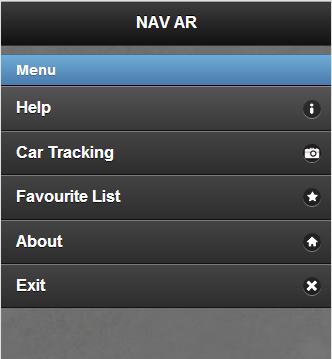
\includegraphics[width=0.5\linewidth]{graphics/chapter4/1}
\caption{Start menu}
\end{figure}


Each one of these buttons have their logic that is implemented in \textbf{index.html}. The listing 4.1 shows the functionality behind each button.
\\

\begin{lstlisting}[language=html, caption= 
Start menu source code,captionpos=b]
<li data-icon="info">
  <a href="help.html" rel="external">
    Help
  </a>
</li>
<li data-icon="camera">
  <a href="#" onclick="trackClick();">
    Car Tracking
  </a>
</li>
<li data-icon="star">
  <a href="myfavourite.html" rel="external">
    Favourite List
  </a>
</li>
<li data-icon="home">
  <a href="about.html" rel="external">
    About
  </a>
</li>
<li data-icon="delete">
  <a href="#" onclick="turnOff();">
    Exit
  </a>
</li>
\end{lstlisting}


\
\
Functions \textit{trackClick()} and \textit{turnOff()} were implemented in Android Java and are described in chapter 5)''Implementation in Android Java and Metaio Tracking''.
\\


\begin{lstlisting}[language=html, caption= 
JavaScript functions in start menu,captionpos=b]
function trackClick() {
    MyTracking.performClick();
}

function turnOff(){
	Exit.exitClick();
}
\end{lstlisting}


The button \textbf{help} forwards the user to the help display \textit{help.html}. The same functionality features \textbf{about} and \textbf{favourite list}, except they link to another display. 
\\

\textbf{Exit} button invokes the function \textit{turnOff()} which calls another Android Java implemented function. \textit{Exit.exitClick()} ends the application. Illustrated in listing 4.2.
\\

\textbf{Car tracking} calls a function \textit{trackClick()}. This method starts the main function.
\\
\newpage


\subsection{Help}
The help display provides only two major options: back button and the link to a tutorial video. This tutorial was created by the project members and is an YouTube video.


\begin{figure}[h]
\centering
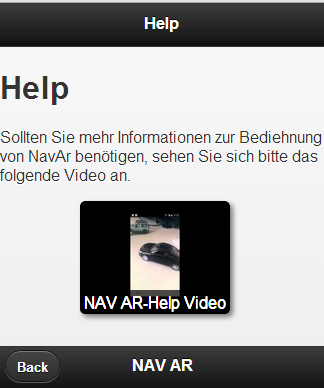
\includegraphics[width=0.5\linewidth]{graphics/chapter4/2}
\caption{Help display}
\end{figure}


The back button leads to the main menu. Shown in listing 4.3.
\\
\begin{lstlisting}[language=html, caption= 
Back button,captionpos=b]
<a class="ui-btn-left" href="index.html" rel="external">
	Back
</a>
\end{lstlisting}
\
\


If the user touches the picture \textbf{NAV AR - Help Video}, he will be linked to a specific how-to YouTube video. This video serves as a simple help to understand how the application works. It shows how to use the application's main functions and more.
\\

\begin{lstlisting}[language=html, caption= 
Help video,captionpos=b]
<a href="https://www.youtube.com/watch?v=6U4oT5AbAsg&feature">
  NAV AR-Help Video
</a>
\end{lstlisting}


%%%%%%%%%%%%%%%%%%%%%%%%%%%%%%%%%%%%%%%%%%%%%%%%%%%%%%%%%%%%%%%%%%
%New Chapter Main Menu
%%%%%%%%%%%%%%%%%%%%%%%%%%%%%%%%%%%%%%%%%%%%%%%%%%%%%%%%%%%%%%%%%
\subsection{Main Menu}
The most important function of the whole mobile applications is \textbf{car tracking}. This function is executed by \textit{MyTracking.peformClick()}. More in chapter 4.1)''Start Menu''.
\\

After a car was successfully tracked, the user is linked to a new display called \textbf{index.html}, which is the start menu. It provides the user with additional options. Options that deliver technical information as well as review about the tracked car and more other useful functions. 
\\

There is also a possibly to add the tracked car to users car collection named \textbf{the favourite list}. Out of there he can select one specific vehicle to use the start menu options, like picture or videos gallery.
\\

JavaScript functions had to be created for each  of this options. These functions are described in chapter 4.3.1)''JavaScript Functions''.
\\

\begin{figure}[h]
\centering
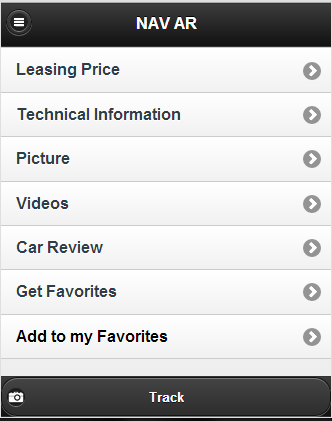
\includegraphics[width=0.5\linewidth]{graphics/chapter4/3}
\caption{Main Menu}
\end{figure}
\newpage


\
Listing 4.23 shows the function behind each button. Some buttons only link to another, other invoke specific functions like \textit{LocalStorageWriteId()}.\\
\begin{lstlisting}[language=html, caption= 
GUI source code,captionpos=b]
<ul data-role="listview" >	
  <li>
    <a href="leasingprice.html" rel="external">
      Leasing Price
    </a>
  </li>
  <li>
    <a href="technicalinfo.html" rel="external">
      Technical Information
    </a>
  </li>
  <li>
    <a href="slide.html" data-transition="slide"rel="external">
      Picture
    </a>
  </li>
  <li>
    <a href="video.html" rel="external">
      Videos
    </a>
  </li>
  <li>
    <a href="#" rel="#" onclick="reviewClick();">
      Car Review
    </a>
  </li>
  <li>
    <a href="myfavourite.html"rel="external">
      Get Favorites
    </a>
  </li>
  <li>
    <a id="add_favorite" 
    onclick="LocalStorageWriteId(sessionStorage.getItem('id'),
    globalcarname);" style="color:red" rel="external">
      Add to my Favorites
    </a>
  </li>
</ul>
\end{lstlisting}
\newpage


\subsubsection{Leasing Price}
%%%%%%%%%%%%%%%%%%%%%%%%%%%%%%%%%%%%%%%%%%%%%%%%%%%%%%%%%%%%%%%%%%%%
%link to chapter with leasing price technologie
%%%%%%%%%%%%%%%%%%%%%%%%%%%%%%%%%%%%%%%%%%%%%%%%%%%%%%%%%%%%%%%%%%%%
When the user presses on button \textbf{leasing price} he will be linked to the html page \textit{leasingprice.html} where he receives informations about the specific vehicle. \\
\
\

\begin{figure}[h]
\centering
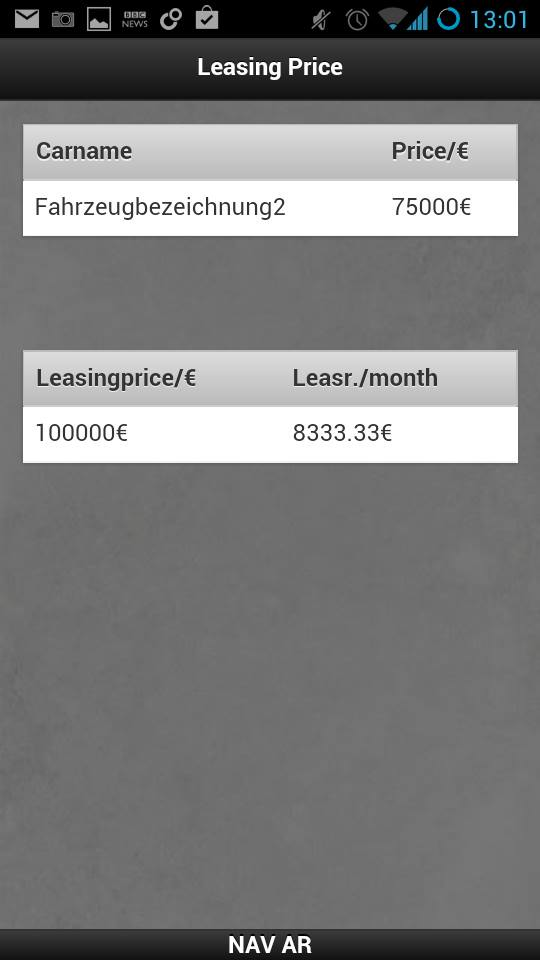
\includegraphics[width=0.5\linewidth]{graphics/chapter4/5}
\caption{Leasing Price}
\end{figure}
\newpage


\subsubsection{Technical Information}
By calling \textbf{technical information} facts about a specific car are presented. To create it several new features had to be used. Phone Gallary and Dynamic Selection of Colour. Informations about those are featured in chapters 4.6)''Photo Gallery'' and  4.8)''Dynamic Selection of Colours''.
\\

\begin{figure}[h]
\centering
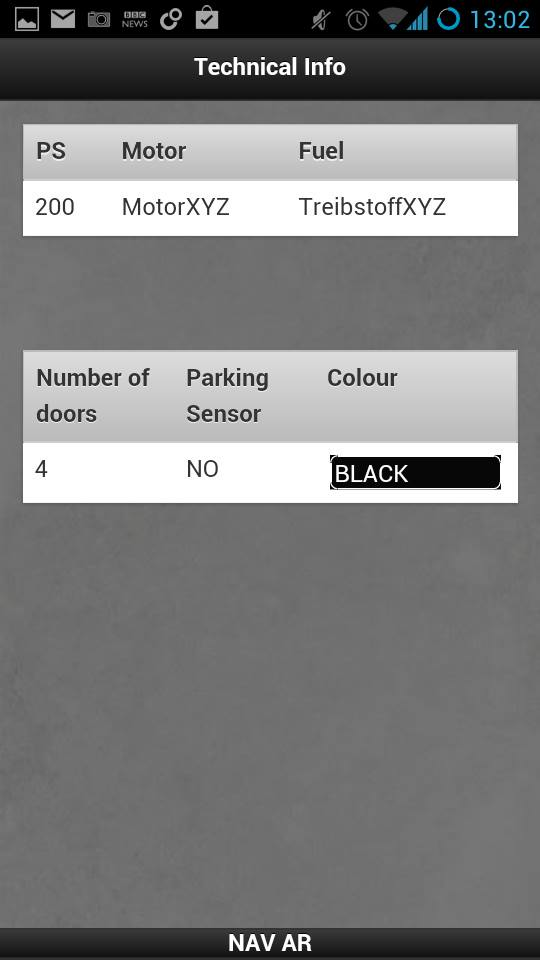
\includegraphics[width=0.5\linewidth]{graphics/chapter4/6}
\caption{Technical Information}
\end{figure}
\newpage

\subsubsection{Pictures}
Has freshest pictures of the specific car. Feature called Photo Gallery in chapter ..... was used to create this option.

\begin{figure}[h]
\centering
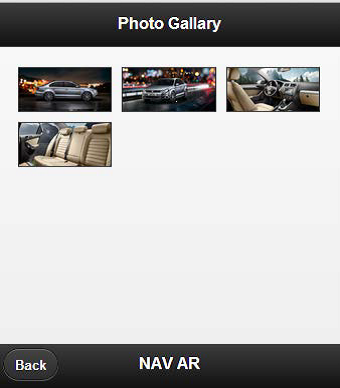
\includegraphics[width=0.5\linewidth]{graphics/chapter4/7}
\caption{Pictures}
\end{figure}
\newpage

\subsubsection{Videos}
This option provides the user with videos about the selected car from favourite list or fresh tracked one. More about video gallery in chapter.....
\\
\begin{figure}[h]
\centering
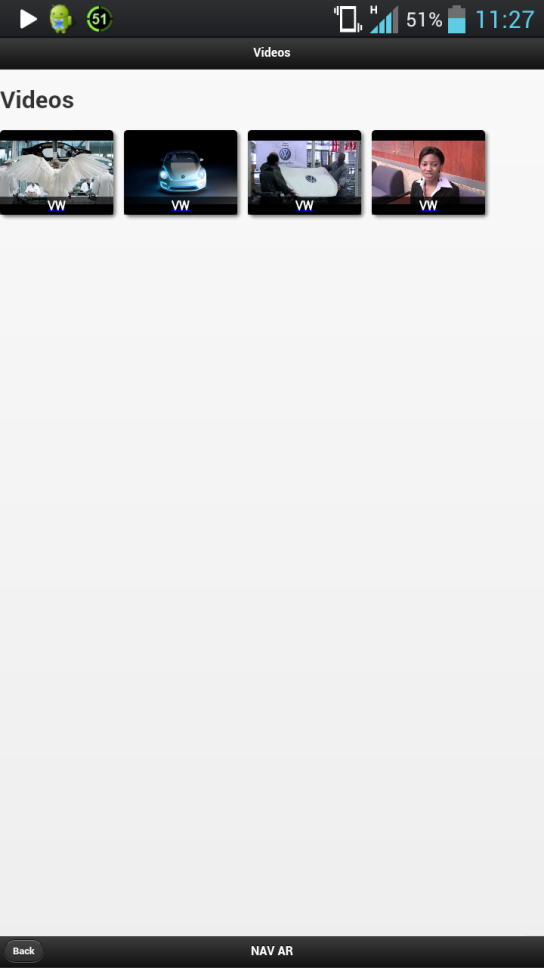
\includegraphics[width=0.5\linewidth]{graphics/chapter4/8}
\caption{Video Gallery}
\end{figure}
\newpage

\subsubsection{Review}
Operation review invokes a self created method called \textit{reviewClick()}. Description to thisit is in chapter 4.3.1 Created Methods, Review. Basically review links the user to a new display where he can read review about the specific car.
\\

\begin{figure}[h]
\centering
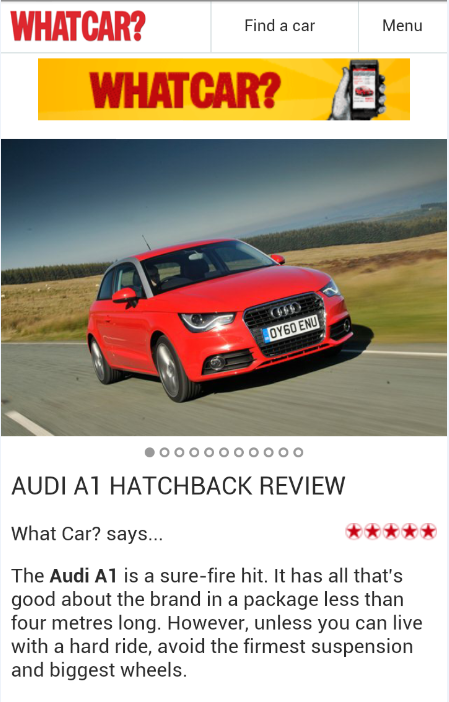
\includegraphics[width=0.5\linewidth]{graphics/chapter4/9}
\caption{}
\end{figure}
\newpage


\subsubsection{Get Favourites}
This operations links the user to his favourite cars which he saved with the option \textbf{add to my favourite}. Information about the favourite list in chapter 4.4)My Favourites.
\\

\begin{figure}[h]
\centering
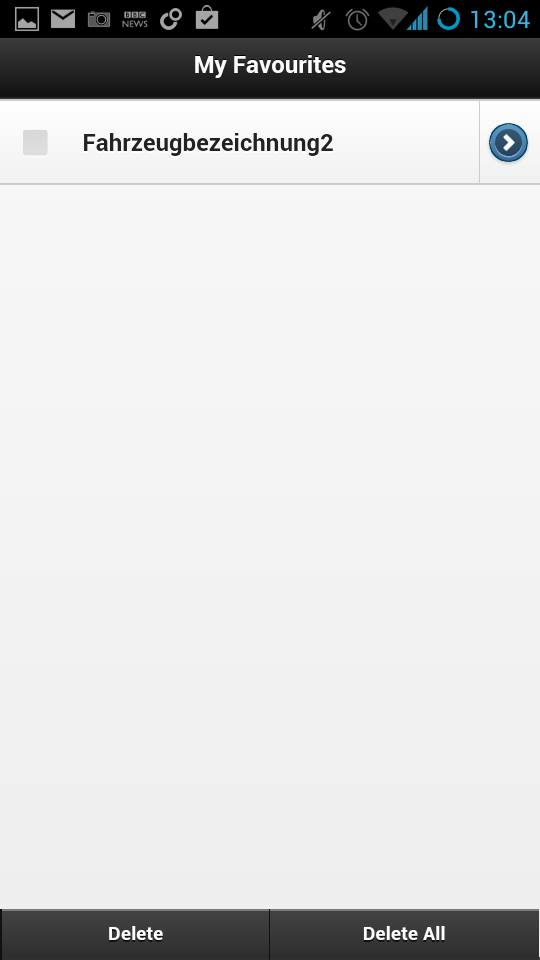
\includegraphics[width=0.5\linewidth]{graphics/chapter4/10}
\caption{Favourite list}
\end{figure}
\newpage

\subsubsection{Add to my Favourites}
The button \textbf{Add to my Favourites} trigger the function \textit{LocalStorageWriteId()}. It saves the id and the name of the tracked car into users favourites. For the first parameter it takes the tracked car id from the session storage. For the second parameter the global variable \textit{globalcarname}.
\\

\begin{lstlisting}[language=html, caption= 
add favourite sorce code,captionpos=b]
<li>
  <a id="add_favorite"onclick="LocalStorageWriteId
  (sessionStorage.getItem('id'),globalcarname);"
  style="color:red" rel="external">
    Add to my Favorites
   </a>
</li>
\end{lstlisting}
\

\
Before the user can add the vehicle to his favourites he has to wait several seconds. In this time the request is send to the server for information about the car threw its id. If the user wants to access the operation in its loading time, the application denies him the access and informs him about the loading time.
\\

\begin{figure}[h]
\centering

\includegraphics[width=0.65\linewidth]{graphics/chapter4/11}
\caption{Not ready function}
\end{figure}
\

The operations colour changes from red to black when the function is loaded.
\\
\begin{figure}[h]
\centering

\includegraphics[width=0.65\linewidth]{graphics/chapter4/12}
\caption{Ready function}
\end{figure}
\newpage

\subsection{My Favourites}
Inside the favourites are cars had been added threw the operation \textbf{add to my favourites}. The favourite cars can be selected or deleted. Removing the cars from favourites is possible by selecting the specific vehicle or removing all of the cars.
\\

\begin{figure}[h]
\centering
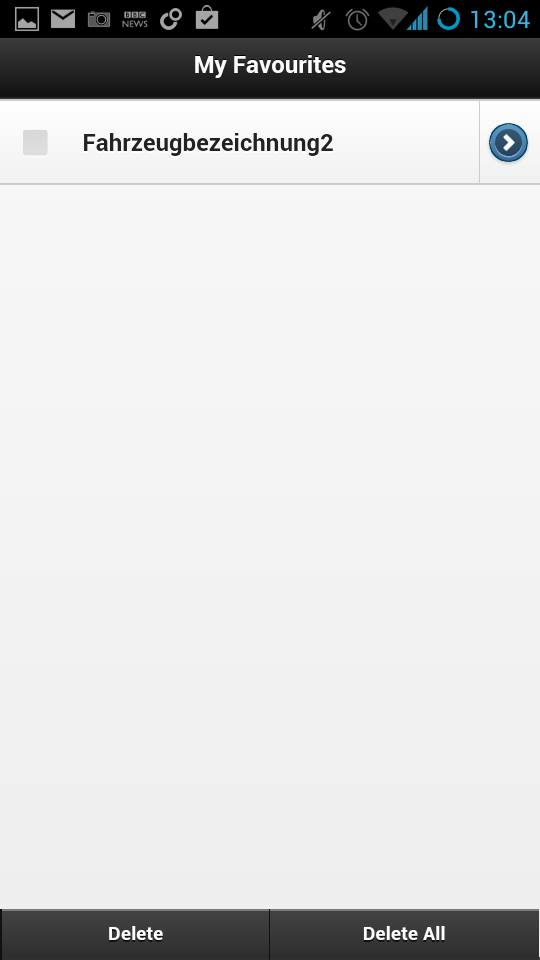
\includegraphics[width=0.4\linewidth]{graphics/chapter4/15}
\caption{My Favourites display}
\end{figure}
\



\subsubsection{Loading of favourite cars}
Before the functions of the favourite list can be used, the list entries(cars) have to be initialized. This is done automatically when the site is loaded. 
\\

Each line that is written inside document.ready starts after the document is ready. This is where the favourite cars are initialized.
\\
\newline
\newline

\begin{lstlisting}[language=html, caption= 
source for document is ready,captionpos=b]
$(document).ready(function () {
.
});
\end{lstlisting}
\

First, all car names are loaded from local storage into an array called \textit{storedCarNames}. So this array is filled with vehicle names which user added to his favourites. 
\\

\begin{lstlisting}[language=html, caption= 
Array with favourite cars,captionpos=b]
var storedCarNames = JSON.parse(localStorage["fcarname"]); 
\end{lstlisting}
\


Now the filling of the cars into a list begins. The loop goes so long as the number of cars in the array. In this loop a car name is put into the \textit{listItem1} which is just a panel shown in figure 4.17.
\\

Next \textit{listItem1} is put into another list. This list is where all panels(favourite cars) are stored. Each new vehicle is put into the list.
\\
\begin{lstlisting}[language=html, caption= 
Adding list items into the list,captionpos=b]
for (var i = 0; i < storedCarNames.length; i++){
  var key = storedCarNames[i];
  listItem1 = '"specific list item"';

  $('#liste').append(listItem1);
}
\end{lstlisting}

\begin{figure}[h]
\centering

\includegraphics[width=0.7\linewidth]{graphics/chapter4/16}
\caption{A list item}
\end{figure}

Last but not least the list that has to be refreshed so the list items are displayed. 
\\

\begin{lstlisting}[language=html, caption= 
Refreshing the list,captionpos=b]
$('#liste').listview('refresh').trigger('create'); 
\end{lstlisting}


\subsection{About}
The \textbf{about} display has no logic and no self made functions except one the back button which functionality you have learnt in 4.2)Help chapter.
\\
\begin{figure}[h]
\centering
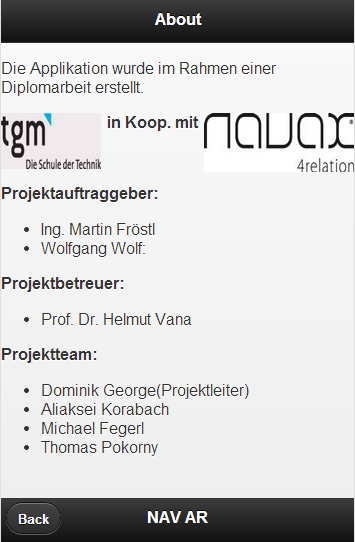
\includegraphics[width=0.4\linewidth]{graphics/chapter4/17}
\caption{About display}
\end{figure}
\newpage


\section{Implemented Function}


\subsection{Start timer}
When the site is loaded a timer automatically starts. Specific functions stop the timer and sends the time stamp to the NAV server.
\\
\begin{lstlisting}[language=html, caption= 
Start timer function,captionpos=b]
function startTime(){
	var d = new Date();
	timestart = d.getTime();
}
\end{lstlisting}

\subsection{End timer}
This function stops the timer which had been started with the method \textit{startTime()} and safes the time with the method \textit{timestampsave()}. The timer was used to get the time how long a user has selected a specific car and used certain start menu options.
\\

\begin{lstlisting}[language=html, caption= 
End timer function,captionpos=b]
function endtime(){
	var d = new Date();
	var endtime = d.getTime();
	timestampsave(timestart,endtime);
}
\end{lstlisting}


\subsection{Save the time}
This function saves start time and end time of the timer, into the NAV server. The start time and end time are the input parameters. 
\\

%%%%%%%%%%%%%%%%%%%%%%%%%%%%%%%%%%%%%%%%%%%%%%%%%%%%%%%%%%%%%%%%%%
%link to michaels chapter about the connection
%%%%%%%%%%%%%%%%%%%%%%%%%%%%%%%%%%%%%%%%%%%%%%%%%%%%%%%%%%%%%%%%%%

To save the time into the server \textit{timestampsave()} needs several other information like email and id of the tracked car. More about sending information to the server and  to the connectivity between application and server read the chapter 7.0.3.4)''Communication from mobile device to the C App''.
\\

time1.....start time
\\
time2.....end time\\
\newline


\begin{lstlisting}[language=html, caption= 
Save time function,captionpos=b]
function timestampsave(time1,time2){
  var stime	= time1;
  var endtime = time2;
  var emailan = sessionStorage.getItem('email');
  var fid = sessionStorage.getItem('id');
    
  $(document).ready(function () {
     $.ajax({
        type: "GET",
        url: "URL",
        async: false,
        dataType: 'JSONP',
        success: function(data){
        //do your stuff with the JSON data
          var test=data;
          console.log(test);
        }
     });
  });
}
\end{lstlisting}


\subsection{Set parameters}
There are two parameters that have to be saved into the session storage to establish a connection with the NAV server. That were id of the tracked car and the email address of the user.
\\
\begin{lstlisting}[language=html, caption= 
Set parameter function,captionpos=b]
function setParam(){
	window.sessionStorage.setItem('id', myVariable);
	window.sessionStorage.setItem('email',email);
}
\end{lstlisting}

%%%%%%%%%%%%%%%%%%%%%%%%%%%%%%%%%%%%%%%%%%%%%%%%%%%%%%%%%%%%%%%%%%
%link to chapter with car tracking in java android
%%%%%%%%%%%%%%%%%%%%%%%%%%%%%%%%%%%%%%%%%%%%%%%%%%%%%%%%%%%%%%%%%%
\subsection{Start car tracking}
This function starts to track a car. For more explanation refer to chapter 5)'Implementation in Android Java and Metaio Tracking'.
\\
\newline
\newline
\begin{lstlisting}[language=html, caption= 
Car tracking function,captionpos=b]
function trackClick() {
  MyTracking.performClick();
}
\end{lstlisting}

%%%%%%%%%%%%%%%%%%%%%%%%%%%%%%%%%%%%%%%%%%%%%%%%%%%%%%%%%%%%%%%%%
%link to chapter with the revie in android java
%%%%%%%%%%%%%%%%%%%%%%%%%%%%%%%%%%%%%%%%%%%%%%%%%%%%%%%%%%%%%%%%%
\subsection{Review}
This method is implemented with Java Android. More about in chapter 5)'Implementation in Android Java and Metaio Tracking'.
\\

\begin{lstlisting}[language=html, caption= 
Review function,captionpos=b]
function reviewClick(){
        Review.performClick();
    }
\end{lstlisting}

%%%%%%%%%%%%%%%%%%%%%%%%%%%%%%%%%%%%%%%%%%%%%%%%%%%%%%%%%%%%%%%%%
%link to chapter java android implementation
%%%%%%%%%%%%%%%%%%%%%%%%%%%%%%%%%%%%%%%%%%%%%%%%%%%%%%%%%%%%%%%%%
\subsection{Turn off}
This function is implemented with Android Java and has been documented in 4.1)''Start Menu''.
\\

\begin{lstlisting}[language=html, caption= 
Turn off funtion,captionpos=b]
function turnOff(){
        Exit.performClick();
    }
\end{lstlisting}


\subsection{Home}
This function returns the user back to the start menu and is implemented with Android Java.\\

\begin{lstlisting}[language=html, caption= 
Home function,captionpos=b]
function home(){
        Home.performClick();
    }
\end{lstlisting}


\subsection{Read car name}
This method returns the name of the car that had been tracked threw a car specific id. Each transport has its own unique id. This id is predefined and set after the tracking was successful. Later it is stored in session storage.
\\
\newline  
%%%%%%%%%%%%%%%%%%%%%%%%%%%%%%%%%%%%%%%%%%%%%%%%%%%%%%%%%%%%%%%%%%
%link to chapter with ajax
%%%%%%%%%%%%%%%%%%%%%%%%%%%%%%%%%%%%%%%%%%%%%%%%%%%%%%%%%%%%%%%%%%
So the input parameter \textit{cname} is that specific id of the tracked or selected car. The name of the car is stored in the NAV server. A request had to be send to receive the name. More about Connectivity in chapter 7)''Streaming''.
\\

%%%%%%%%%%%%%%%%%%%%%%%%%%%%%%%%%%%%%%%%%%%%%%%%%%%%%%%%%%%%%%%%%%
%set code on one line
%%%%%%%%%%%%%%%%%%%%%%%%%%%%%%%%%%%%%%%%%%%%%%%%%%%%%%%%%%%%%%%%%%

\begin{lstlisting}[language=html, caption= 
Read car name function,captionpos=b]
function readcarname(cname){
  var test = '';
  $(document).ready(function () {
    $.ajax({
      type: "GET",
        url:"URL",
        async: false,
        dataType: 'JSONP',
        success: function(data){
          test=data.split(';');
          globalcarname=test[0];
          document.getElementById("add_favorite").
          style.color="black";
        }
    });
  });
}
\end{lstlisting}

%%%%%%%%%%%%%%%%%%%%%%%%%%%%%%%%%%%%%%%%%%%%%%%%%%%%%%%%%%%%%%%%%%
%link to chapter with ajax
%%%%%%%%%%%%%%%%%%%%%%%%%%%%%%%%%%%%%%%%%%%%%%%%%%%%%%%%%%%%%%%%%%
\subsection{Save email}
As the name says, \textit{saveEmail()} saves the email of a user. The information about users email was already stored in session storage through the function \textit{setParam()}. More in chapter 5.4)''Get Email Account from an Android device''.\\

Later this email is send to the NAV server. More about connection between app and server in chapter 7)''Streaming''.
\\

\begin{lstlisting}[language=html, caption= 
Save email function,captionpos=b]
function saveEmail(){    
  var value3 = sessionStorage.getItem('email');
  $(document).ready(function () {
     $.ajax({
     type: "GET",
     url: "URL",
       async: false,
       dataType: 'JSONP',
       success: function(data){
       //do your stuff with the JSON data
         var test=data;
         console.log(test);
       }
     });
  });
}
\end{lstlisting}

\subsection{Save car}
This function saves the id and the name of the tracked vehicle. This method is used for adding new cars to users car collection. In this function a feature called local storage that provides HTML5 for its users, was used. The function can be split into four phases.
\\

Phase one checks if the input parameter \textit{name} is not empty. If it is empty user receives information about it, otherwise it processes with the other phases.

\begin{lstlisting}[language=html, caption= 
Phase one,captionpos=b]
if(name!=null){
.....
}else{
  alert("Function is loading.");
}
\end{lstlisting}
\
\

Phase two is the search phase. It searches for unique local storage place threw specific name \textit{(favorites ,fcarna)} and inspects if the storage with the name exists. If it doesn't exists an empty array is put inside the two local storages, else nothing happens.
\\

\begin{lstlisting}[language=html, caption= 
Phase two,captionpos=b]
if ((localStorage.getItem("favorites") === null) &&
 (localStorage.getItem("fcarname") == null)) {
   var names = [];
   localStorage["favorites"] = JSON.stringify(names);	
   localStorage["fcarname"] = JSON.stringify(names);
}
\end{lstlisting}
\newpage

In phase three variables \textit{storedIds} and \textit{storedNames} are filled with information inside the local storage \textit{favorites} and \textit{fcarname}.
\\

\begin{lstlisting}[language=html, caption= 
Phase three,captionpos=b]
var storedIds = JSON.parse(localStorage["favorites"]);
var storedNames = JSON.parse(localStorage["fcarname"]);
\end{lstlisting}

Phase four checks if the car exists in the local storage. If it does the user receives information that this car already exists in the favourite list, else the id and car name is saved into the local storage.
\\

\begin{lstlisting}[language=html, caption= 
Phase four,captionpos=b]
if(storedIds.indexOf(id)>-1){
  Notifier.error('Car already exists.');
}else{
  storedIds.push(id);
  storedNames.push(name);
  localStorage["favorites"] = JSON.stringify(storedIds);
  localStorage["fcarname"] = JSON.stringify(storedNames);
  Notifier.success('Car has been added.');
}
\end{lstlisting}

The listing 4.19 shows the hole function with its four phases.\\
\begin{lstlisting}[language=html, caption= 
Save car function,captionpos=b]
function LocalStorageWriteId(id,name){
  if(name!=null){
    if((localStorage.getItem("favorites")===null)&&
     (localStorage.getItem("fcarname")==null)){
	  var names = [];
	  localStorage["favorites"] = JSON.stringify(names);
	  localStorage["fcarname"] = JSON.stringify(names);
    }		
    var storedIds = JSON.parse(localStorage["favorites"]);
	var storedNames = JSON.parse(localStorage["fcarname"]);	
	if(storedIds.indexOf(id)>-1){
	  Notifier.error('Car already exists.');
	}else{
	  storedIds.push(id);
	  storedNames.push(name);
	  localStorage["favorites"] = JSON.stringify(storedIds);
	  localStorage["fcarname"] = JSON.stringify(storedNames);
	  Notifier.success('Car has been added.');
	}
  }else{
    alert("Function is loading.");
  }
}
\end{lstlisting}



\subsection{Delete favourite car}
This method deletes selected car with help of check box. If no car is selected, nothing happens by clicking on the button.
\\

\begin{lstlisting}[language=html, caption= 
Delete function,captionpos=b]
function deleteF(){
	
	Array.prototype.clean = function(deleteValue) {
  		for (var i = 0; i < this.length; i++) {
    		if (this[i] == deleteValue) {         
      			this.splice(i, 1);
				i--;
			}
		}
		return this;
	};
	
	var storedNames = JSON.parse(localStorage["favorites"]); //the ids of cars
    var storedCarNames = JSON.parse(localStorage["fcarname"]); //the names of cars
	var lengthof=0;

	for(var s=0;s<storedNames.length;s++){
		if(document.getElementById(s).checked){
			delete storedNames[s];
            delete storedCarNames[s];
			lengthof++;
		}		
	}
	if(lengthof!=0){
		Notifier.success('Cars deleted.');
	
		storedNames.clean(undefined);
		storedCarNames.clean(undefined);

		localStorage["favorites"] = JSON.stringify(storedNames);
		localStorage["fcarname"] = JSON.stringify(storedCarNames);
	}
	window.location.reload();
}
\end{lstlisting}

\subsection{Delete all favourite cars}
Removes all favourite cars without selecting them.

\begin{lstlisting}[language=html, caption= 
Delete all function,captionpos=b]
function deleteAll(){
    Notifier.success('All cars have been deleted.');
	localStorage.clear();
    window.location.reload();
}
\end{lstlisting}

\subsection{Select favourite car}
Each car inside the favourite list can be selected. After the car is selected, the user is linked to the start menu.
\\

\begin{lstlisting}[language=html, caption=
Select car function,captionpos=b] 
function EventHandler() {
	Notifier.success('Car is selected.');
	var id = this.id;
	
	var storedNames = JSON.parse(localStorage["favorites"]);
	
	for(var i=0; i<storedNames.length;i++){
		if(id==i){
			window.sessionStorage.setItem('id', storedNames[i]);
		}
	}
}
\end{lstlisting}






















\section{Features}
Several new technologies were used to create the start menu. This chapter describes all those technologies. Some are linked to other chapters where they have already been explained. 
\\


\subsection{Local Storage}

HTML5 provides us with a new feature called Web Storage. In other words, with it web pages can store data locally within the user's browser or mobile application.
\\

Earlier, this was done with cookies. However, Web Storage is more secure and faster. The data is not included with every server request, but used ONLY when asked for. It is also possible to store large amounts of data, without affecting the website's performance.\cite{w3school}
\\

The data is stored in name/value pairs, and a web page can only access data stored by itself. Unlike cookies, the storage limit is far larger (at least 5MB) and information is never transferred to the server.\cite{w3school}
\\

HTML5 Web Storage provides two new objects for storing data on the client:
\begin{enumerate}
\item window.localStorage - stores data with no expiration date\cite{w3school}
\item code.sessionStorage - stores data for one session (data is lost when the tab is closed)\cite{w3school}
\end{enumerate}


\begin{figure}[h]
\centering
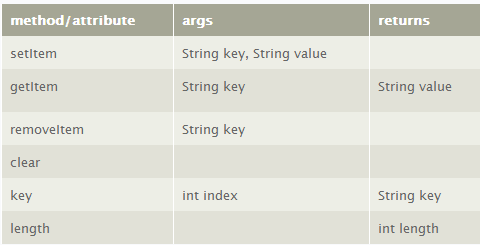
\includegraphics[width=0.9\linewidth]{graphics/chapter4/20}
\caption{Methods and attributes of local storage\cite{localstorageapi}}
\end{figure}


Here is an example of \textit{setItem} and \textit{getItem} in local storage.
\\

\begin{lstlisting}[language=html, caption= 
setItem example (Adapted from \cite{localstorageexample}),captionpos=b]
var foo = localStorage.getItem("bar");
// ...
localStorage.setItem("bar", foo);
\end{lstlisting}

In these application not a string but an array is stored inside the local storage. Here is an example how we put an empty array into a local storage.
\\

\begin{lstlisting}[language=html, caption= 
array into local storage,captionpos=b]
var names = [];
localStorage["favorites"] = JSON.stringify(names);
\end{lstlisting}
\
\

Here an example how we received the array form local storage.
\\
\begin{lstlisting}[language=html, caption= 
start timer function,captionpos=b]
var storedIds = JSON.parse(localStorage["favorites"]);
\end{lstlisting}

\newpage


\subsection{Slide Panel}
%%%%%%%%%%%%%%%%%%%%%%%%%%%%%%%%%%%%%%%%%%%%%%%%%%%%%%%%%%%%%%%%%%%%%
%link to slide panel chapter
%%%%%%%%%%%%%%%%%%%%%%%%%%%%%%%%%%%%%%%%%%%%%%%%%%%%%%%%%%%%%%%%%%%%%
In the upper left corner of the display exists a small button that calls the slide panel to open. More about slide panel in chapter 6.1.0.4)Slide Panel.
\\

\begin{figure}[h]
\centering
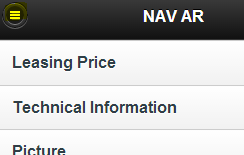
\includegraphics[width=0.5\linewidth]{graphics/chapter4/13}
\caption{Slide panel}
\end{figure}

After opening the slide panel more options are available. 
\\

\begin{figure}[h]
\centering
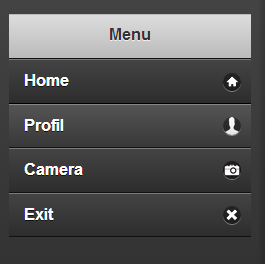
\includegraphics[width=0.5\linewidth]{graphics/chapter4/14}
\caption{Options of slide panel}
\end{figure}
\newpage

Here has the user four new options. He can return to the start menu with the display \textbf{home} or he can accesses his profile with \textbf{profil}. Also he can start to track a new car with \textbf{camera}. If the user doesn't want use the mobile application any more, he can close it the button \textbf{exit}. 
\\
\begin{lstlisting}[language=html, caption=Source code of slide panel options,captionpos=b]
<ul data-role="listview" data-theme="a">
  <li data-icon="home" >
    <a href="#" onclick="endtime();home();">
      Home
    </a>
  </li>
  <li data-icon="profil">
    <a href="profile.html" rel="external">
      Profil
    </a>
  </li>
  <li data-icon="camera" >
    <a href="#" onclick="endtime();trackClick();">
      Camera
    </a>
  </li>
  <li data-icon="delete">
    <a href="#" onclick="endtime();turnOff();">
      Exit
    </a>
  </li>
</ul>
\end{lstlisting}

The \textbf{home} button not only returns the user to the start menu but also ends the timer that has been started after a car was tracked. In addition, this timer is send straight to the NAV server.  
\\

Display \textbf{profil} calls to another display, in which the user can see his profile data. 
\textbf{Camera} function ends the timer and starts the tracking function. Exit ends the application.
\newpage


\subsection{Photo Gallery}
In this subchapter it describes the functionality of the photo gallery . The photo gallery is a feature of this project NAVAR. This feature shows the picture of the car which has been tracked by the NAVAR App. The Photo gallery is a plugin  from the photo swipe webpage. The Logic of the Photo swipe is implemented in a javaScript Library from photo swipe$\rightarrow$ klass.min.js. The functionality of the Design is defined in a css file$\rightarrow$ photoswipe.css. In this project it combined the Library form the photo swipe with the Library from jQuery Mobile. Furthermore the Table shows a Code snippet how to use the Library for this project:
\begin{figure}[htbp]
\centering
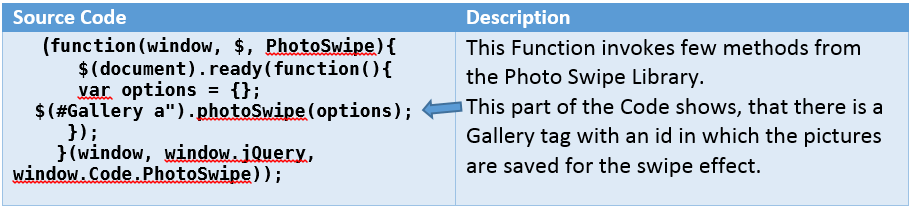
\includegraphics[width=1.0\linewidth]{graphics/photoswipe.PNG}
\caption{Photoswipe}
\end{figure}

Furthermore the pictures are saved on a server and in the Gallery we saved the URL of these pictures. The URL's are saved in an Array which has the id Gallery. For each car there is an Array with URL's of the pictures. Besides the photo swipe has the function to set a automatic Diashow.\\\\

\subsection{Sessionstorage}
Moreover the function called Sessionstorage is one of the big functionalities in this project. The Sessionstorage saves the value not persist, it means if the App is closed or has been ended  the value will be persistant . In the next Session or if the App has been started , there will be a new Sessionstorage. In this case the Project NAVAR uses the Sessionstorage to save the ID from the car, which has been tracked. Sessionstorage allows  to save a large amount of  key/value pairs and lots of text. This feature is impossible to do  via cookie. This kind of functionality uses  a protocol to save the Data. This protocol checks if the key and the value are a string, but if not it convert them to a string. Furthermore if a key was already present, its entry  has to be removed and the new one will be appended. The SessionStorage has it own methods for specific functionality.\\\\

First method is used to tell how many key/pair the SessionStorage contains. This method has the same function ,which tells the length of an Array, HTMLCollection \dots

\begin{figure}[htbp]
\centering
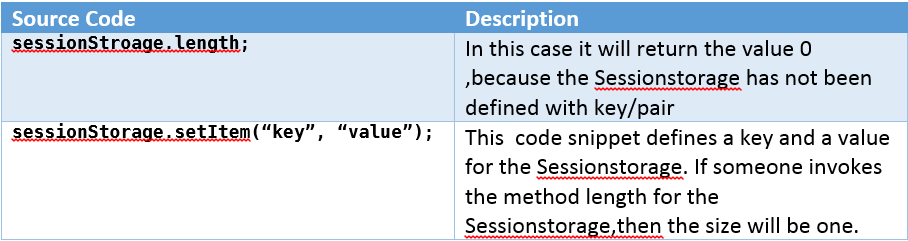
\includegraphics[width=1.0\linewidth]{graphics/sessionstorage1.PNG}
\caption{Sessionstorage}
\end{figure}

The second Method of Sessionstorage is called \textit{setItem(key:string,data:string)}.
 This method stores  a specified key  and the data. But if the key has been already stored and it uses the same key it will be overwritten. $\rightarrow$Example for setItem:\textbf{ sessionStorage.setItem('testkey','testvalue')}.
The third function is to get Data from the a specified key ,which has been already set. This method accepts any sort of string ,which has been used as key and returns the associated string as value or null if the key has not been stored before. Example:\\

\begin{figure}[htbp]
\centering
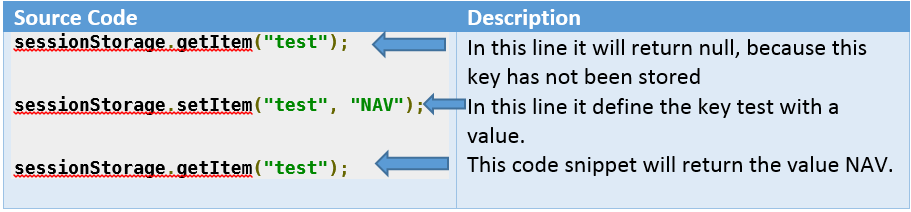
\includegraphics[width=1.0\linewidth]{graphics/sessionstorage2.PNG}
\caption{Sessionstorage}
\end{figure}

The last function is how to remove the key if it has no need for the Session. Example:
\begin{figure}[htbp]
\centering
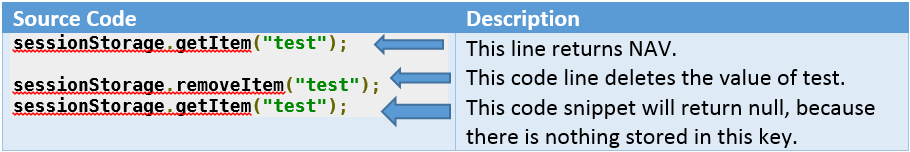
\includegraphics[width=1.0\linewidth]{graphics/sessionstorage3.PNG}
\caption{Sessionstorage}
\end{figure}

\subsection{Dynamic Selection of Colour}
This product has the feature to select the colour of the car . In the Technical Information the user has the opportunity to chose the colour of the Car, which has been tracked. The following code in the Figure shows how to create a dynamic selector with JavaScript:
\begin{figure}[htbp]
\centering
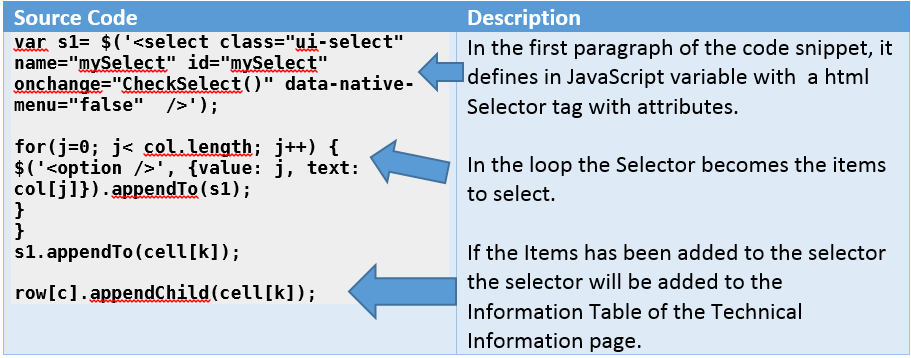
\includegraphics[width=1.0\linewidth]{graphics/Sessionstorage41.PNG}
\caption{Selector descritpion}
\end{figure}
The following picture shows how the Technical Info table looks like:
\begin{figure}[htbp]
\centering
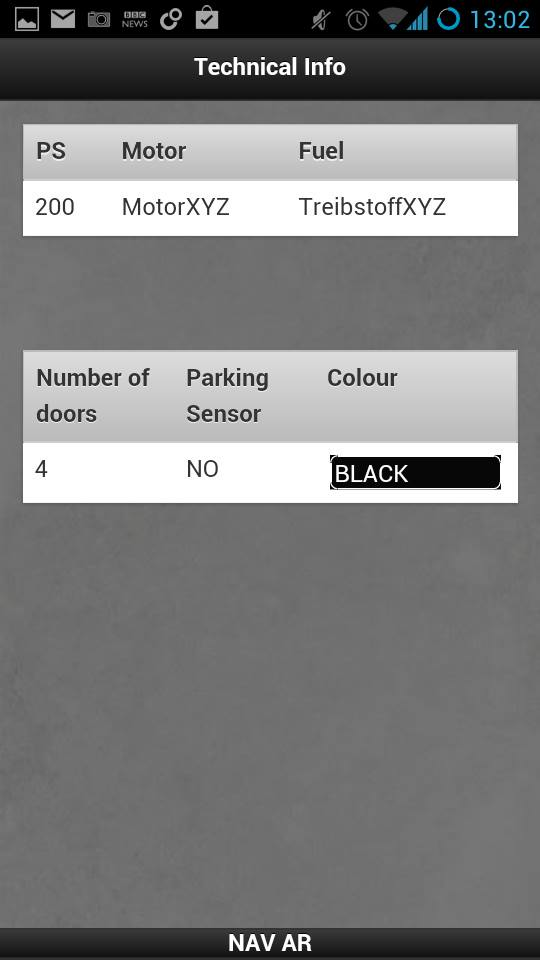
\includegraphics[width=0.4\linewidth]{graphics/chapter4/6.png}
\caption{Table}
\end{figure}
The second picture shows how the dynamic List of items from the Selector looks like:
\begin{figure}[htbp]
\centering
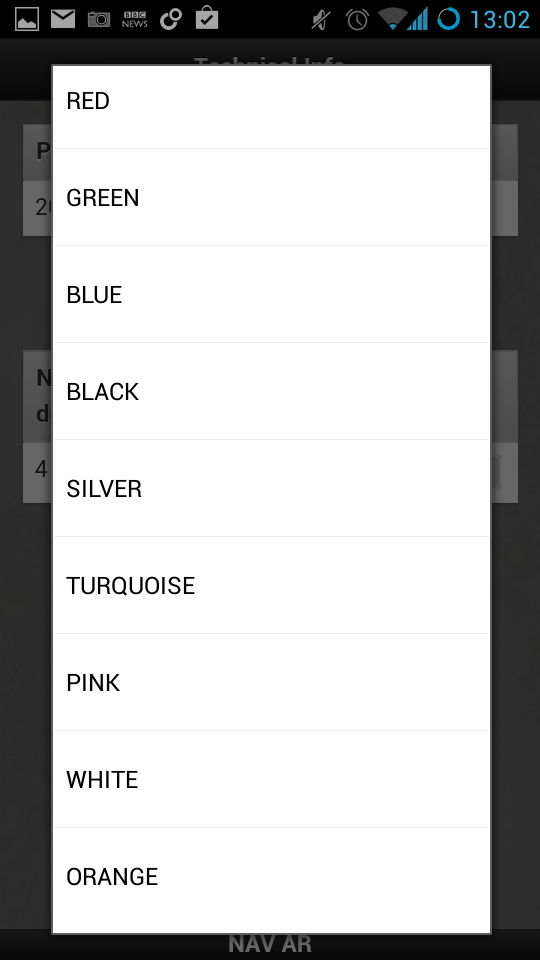
\includegraphics[width=0.4\linewidth]{graphics/chapter4/fg6.png}
\caption{Selector}
\end{figure}
Furthermore there is  a logic implemented which checks if the Colour is white or Black , that changes the colour of the font. The following code snippet shows how to write it:\\
\begin{figure}[htbp]
\centering
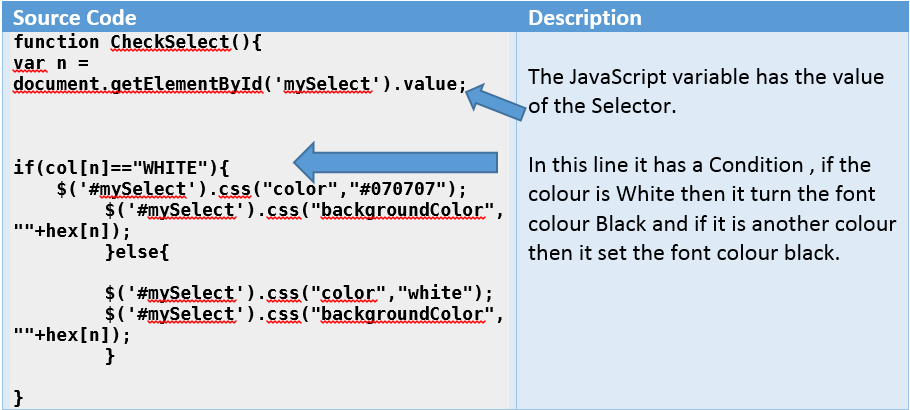
\includegraphics[width=1.0\linewidth]{graphics/bgfn.PNG}
\caption{Condition}
\end{figure}
